
\chapter{Projeto do Sistema}

\section{Arquitetura do Sistema}
A arquitetura do Sistema Web Administrativo da Confeitaria Bom Gosto foi planejada de forma modular, com o objetivo de organizar as funcionalidades e facilitar a comunicação entre as diferentes áreas da aplicação. A estrutura está dividida em dois grandes módulos: o Mega-Componente Administrativo e o Mega-Componente Fábrica.

O Mega-Componente Administrativo reúne as funcionalidades relacionadas ao gerenciamento dos pedidos, à organização das entregas e retiradas, ao controle financeiro e à autenticação do usuário. Já o Mega-Componente Fábrica concentra as operações relacionadas à produção dos produtos, ao controle de ingredientes, ao estoque e à geração de relatórios.

A divisão permite separar as atividades administrativas das atividades operacionais de produção, mantendo a comunicação entre os módulos sempre que uma funcionalidade depende de informações de outra área.

O módulo administrativo, por exemplo, pode consultar a disponibilidade de produtos no estoque e encaminhar uma demanda para produção quando necessário. Da mesma forma, as informações de pedidos e pagamentos podem ser utilizadas para organizar a agenda e acompanhar os registros financeiros.

A Figura~\ref{fig:arquitetura_componentes} apresenta a organização dos componentes e seus relacionamentos.

\begin{figure}[H]
    \centering
    \caption{\label{fig:arquitetura_componentes}Diagrama de componentes do Sistema Web Administrativo da Confeitaria Bom Gosto}
    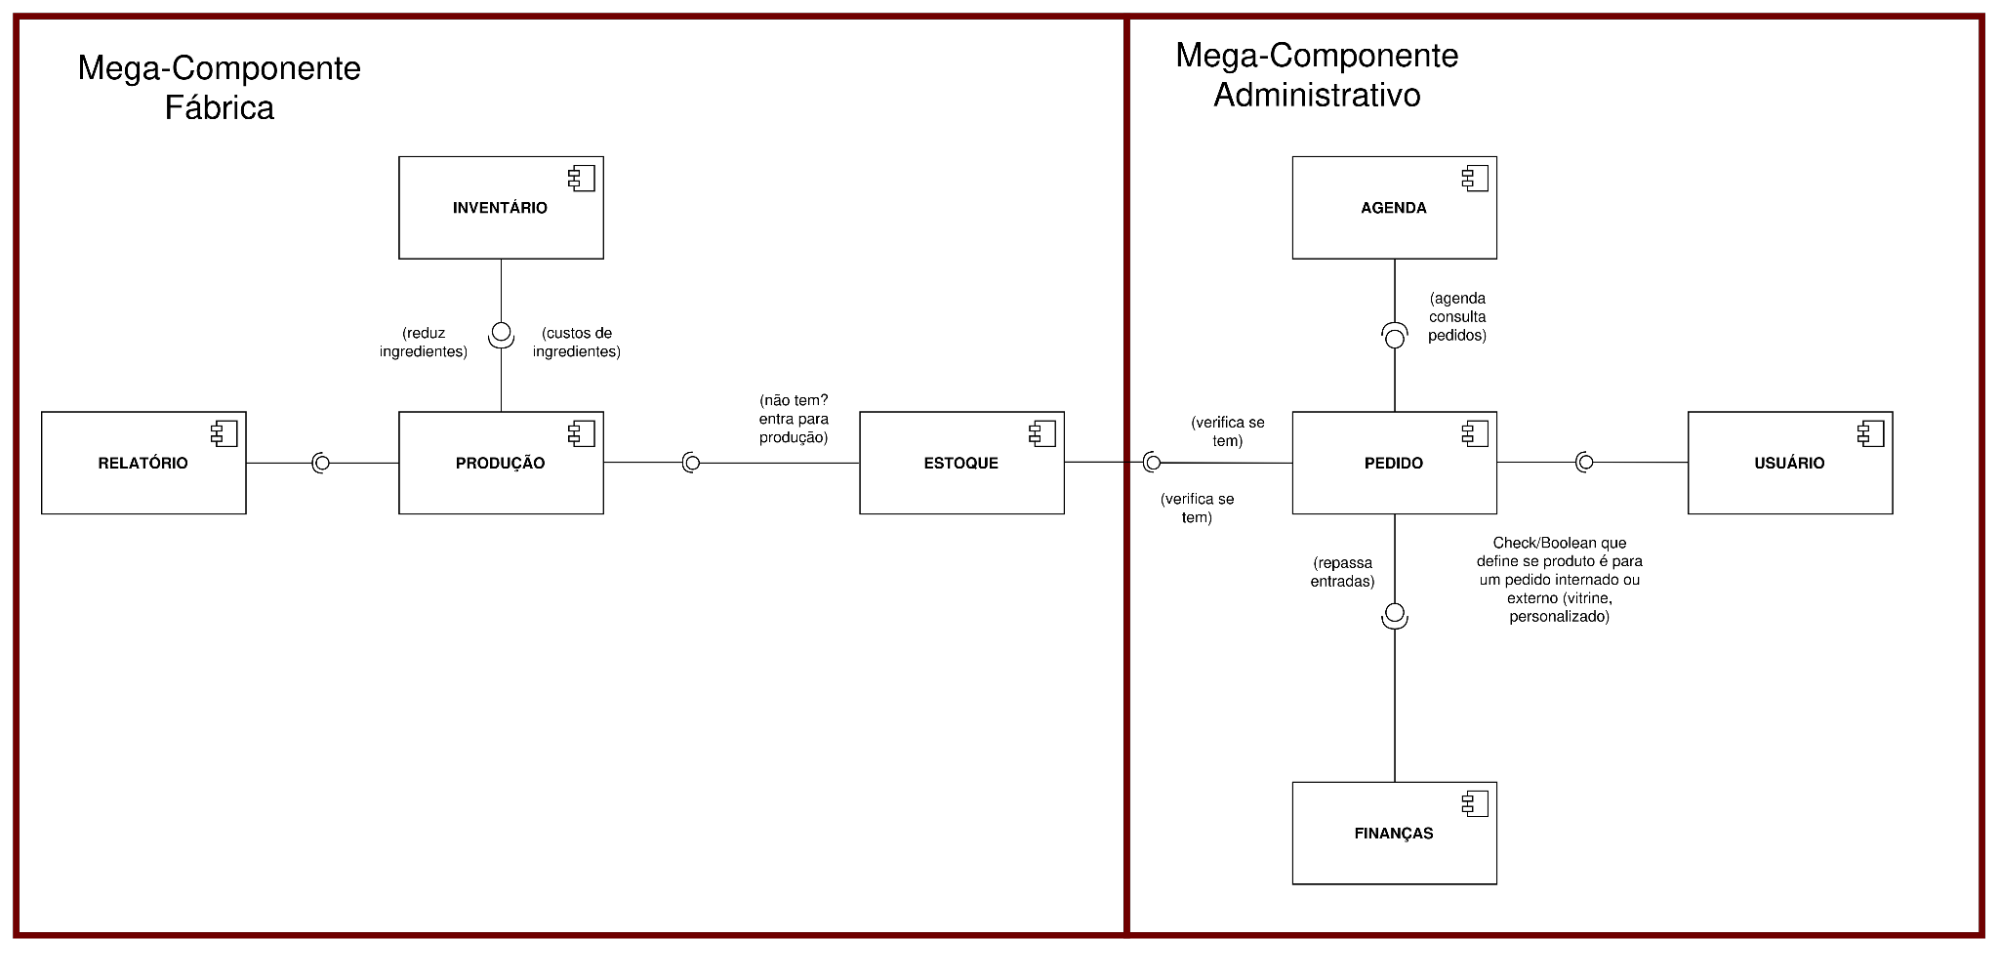
\includegraphics[width=\textwidth]{imagens/diagrama_componentes.png}
    \legend{Fonte: Elaborado pelos autores (2026).}
\end{figure}


\subsection{Mega-Componente Fábrica}

\begin{itemize}
    \item \textbf{Componentes internos:} RELATÓRIO, INVENTÁRIO, PRODUÇÃO e ESTOQUE.
    \item \textbf{Interfaces e relacionamentos:}
    \begin{itemize}
        \item \textbf{Insumos/Ingredientes:} estabelece a relação entre os componentes Inventário e Produção, permitindo que o processo produtivo consulte os ingredientes necessários para a fabricação dos produtos.
        
        \item \textbf{Insere para produção:} representa a comunicação entre Produção e Estoque, permitindo que os produtos fabricados sejam registrados no estoque após sua produção.
    \end{itemize}
\end{itemize}

\subsection*{Mega-Componente Administrativo}

\begin{itemize}
    \item \textbf{Componentes internos:} AGENDA, PEDIDO, FINANÇAS e USUÁRIO.
    
    \item \textbf{Interfaces e relacionamentos:}
    \begin{itemize}
        \item \textbf{Agenda:} consulta as informações dos pedidos para organizar e apresentar as datas e os horários previstos para entregas e retiradas.
        
        \item \textbf{Pedido:} verifica a disponibilidade de insumos e produtos junto ao módulo Fábrica, encaminha as demandas necessárias para produção e estabelece a comunicação com o componente Finanças para o registro das informações de pagamento. Também considera se o produto é destinado a um pedido personalizado ou à vitrine.
        
        \item \textbf{Usuário:} representa o ponto de interação direta com o sistema, permitindo o acesso às funcionalidades administrativas por meio da interface da aplicação.
    \end{itemize}
\end{itemize}


\section{Projeto dos Componentes}

O projeto dos componentes define a responsabilidade de cada módulo e a maneira como suas funcionalidades contribuem para o funcionamento do sistema. Para facilitar a compreensão da estrutura, os componentes foram agrupados de acordo com suas responsabilidades administrativas e operacionais.

\subsection{Mega-Componente Administrativo}

O Mega-Componente Administrativo reúne as funcionalidades utilizadas no gerenciamento cotidiano da confeitaria, abrangendo o registro de encomendas, a organização dos compromissos, o acompanhamento financeiro e o controle de acesso.

\subsubsection{Componente Pedido}

O componente Pedido é responsável pelo gerenciamento das encomendas registradas no sistema. Ele reúne as informações necessárias para identificar o pedido, como os dados do cliente, o produto solicitado, as especificações de personalização, a data e o horário previstos para entrega ou retirada e as condições de pagamento.

O componente também permite distinguir pedidos destinados ao atendimento de clientes daqueles relacionados à reposição de produtos para a vitrine. No caso das encomendas externas, é possível diferenciar produtos de vitrine e produtos personalizados.

Além disso, o componente se relaciona com o Estoque, para consultar a disponibilidade dos produtos, com a Agenda, para organizar os compromissos, e com Finanças, para registrar as informações referentes aos pagamentos.

\subsubsection{Componente Agenda}

O componente Agenda é responsável pela organização temporal dos pedidos. Ele reúne as datas e os horários associados às entregas e retiradas, permitindo consultar os compromissos previstos para determinado período.

As informações são obtidas a partir dos pedidos cadastrados, contribuindo para o planejamento das atividades diárias e semanais da confeitaria. Dessa forma, a agenda auxilia na visualização dos prazos e na organização da produção.

\subsubsection{Componente Finanças}

O componente Finanças concentra os registros financeiros relacionados às atividades da confeitaria. Ele considera os pagamentos parciais, como os sinais de encomendas, os pagamentos totais e as despesas registradas com a aquisição de ingredientes e outros insumos.

A organização dessas informações permite acompanhar os recebimentos e as despesas e fornece dados para a consulta do faturamento e dos resultados financeiros. A precisão dos resultados depende do preenchimento correto e da atualização dos registros.

\subsubsection{Componente Usuário}

O componente Usuário é responsável pela autenticação e pelo controle de acesso à aplicação. Como o sistema foi planejado para utilização administrativa pela proprietária da confeitaria, seu acesso deve ser restrito à pessoa autorizada.

Esse componente está relacionado à validação das credenciais e à proteção das funcionalidades administrativas, de acordo com os mecanismos de segurança efetivamente implementados.

\subsection{Mega-Componente Fábrica}

O Mega-Componente Fábrica reúne as funcionalidades relacionadas à produção, ao gerenciamento de matérias-primas, ao controle de produtos disponíveis e à análise dos dados operacionais.

\subsubsection{Componente Estoque}

O componente Estoque é responsável pelo controle da quantidade de produtos prontos disponíveis para venda ou entrega imediata, incluindo os itens destinados à vitrine.

Quando um pedido exige determinado produto, o componente permite verificar sua disponibilidade. Caso a quantidade registrada não seja suficiente, a necessidade poderá ser encaminhada ao processo de produção, conforme as regras definidas para o sistema.

\subsubsection{Componente Produção}

O componente Produção concentra as informações necessárias à fabricação dos produtos da confeitaria. Ele relaciona os produtos às respectivas receitas, considerando os ingredientes e as quantidades utilizadas em cada preparação.

Essas informações permitem estimar os custos das receitas e organizar as necessidades de fabricação. O processo de produção também se relaciona com o Inventário, para consultar e atualizar as quantidades de ingredientes, e com o Estoque, para registrar os produtos fabricados.

\subsubsection{Componente Inventário}

O componente Inventário é responsável pelo controle das matérias-primas e dos ingredientes utilizados na produção. Seus registros contemplam informações como a identificação do insumo, a quantidade disponível, o custo de aquisição e a data de validade.

O componente fornece informações para o planejamento da produção e para o acompanhamento dos custos dos ingredientes. Quando ocorre o consumo de matérias-primas, as quantidades do inventário devem ser atualizadas de acordo com o processo implementado na aplicação.

\subsubsection{Componente Relatório}

O componente Relatório reúne informações provenientes das operações de produção, do inventário e dos demais registros disponíveis no sistema.

Sua finalidade é apoiar a análise das atividades da confeitaria, permitindo consultar informações como os custos de produção, o consumo de ingredientes e os resultados registrados. A disponibilidade de cada indicador depende dos dados armazenados e das funcionalidades implementadas.

\section{Modelo de Dados}

O modelo de dados define como as informações utilizadas pelo Sistema Web Administrativo da Confeitaria Bom Gosto são organizadas e relacionadas. Sua finalidade é estabelecer uma estrutura consistente para o armazenamento e a consulta dos registros necessários às funcionalidades da aplicação.

O modelo considera informações relacionadas aos usuários, clientes, pedidos, itens dos pedidos, pagamentos, produtos, estoque, receitas, ingredientes, produção e movimentações de inventário. A organização dessas informações busca reduzir duplicidades desnecessárias e manter os relacionamentos necessários entre os registros.

A modelagem pode ser compreendida em três níveis. O modelo conceitual representa as principais entidades do domínio e seus relacionamentos. O modelo lógico detalha a organização dos dados e as relações entre as entidades. Por fim, o modelo físico corresponde à estrutura definida no sistema gerenciador de banco de dados utilizado pela aplicação.

Essa separação contribui para a compreensão da estrutura dos dados e permite relacionar as informações armazenadas às funcionalidades descritas nas etapas anteriores do projeto.

A Figura~\ref{fig:modelo_dados} apresenta o modelo lógico de dados do sistema.

\begin{figure}[H]
    \centering
    \caption{\label{fig:modelo_dados}Modelo lógico de dados do Sistema Web Administrativo da Confeitaria Bom Gosto}
    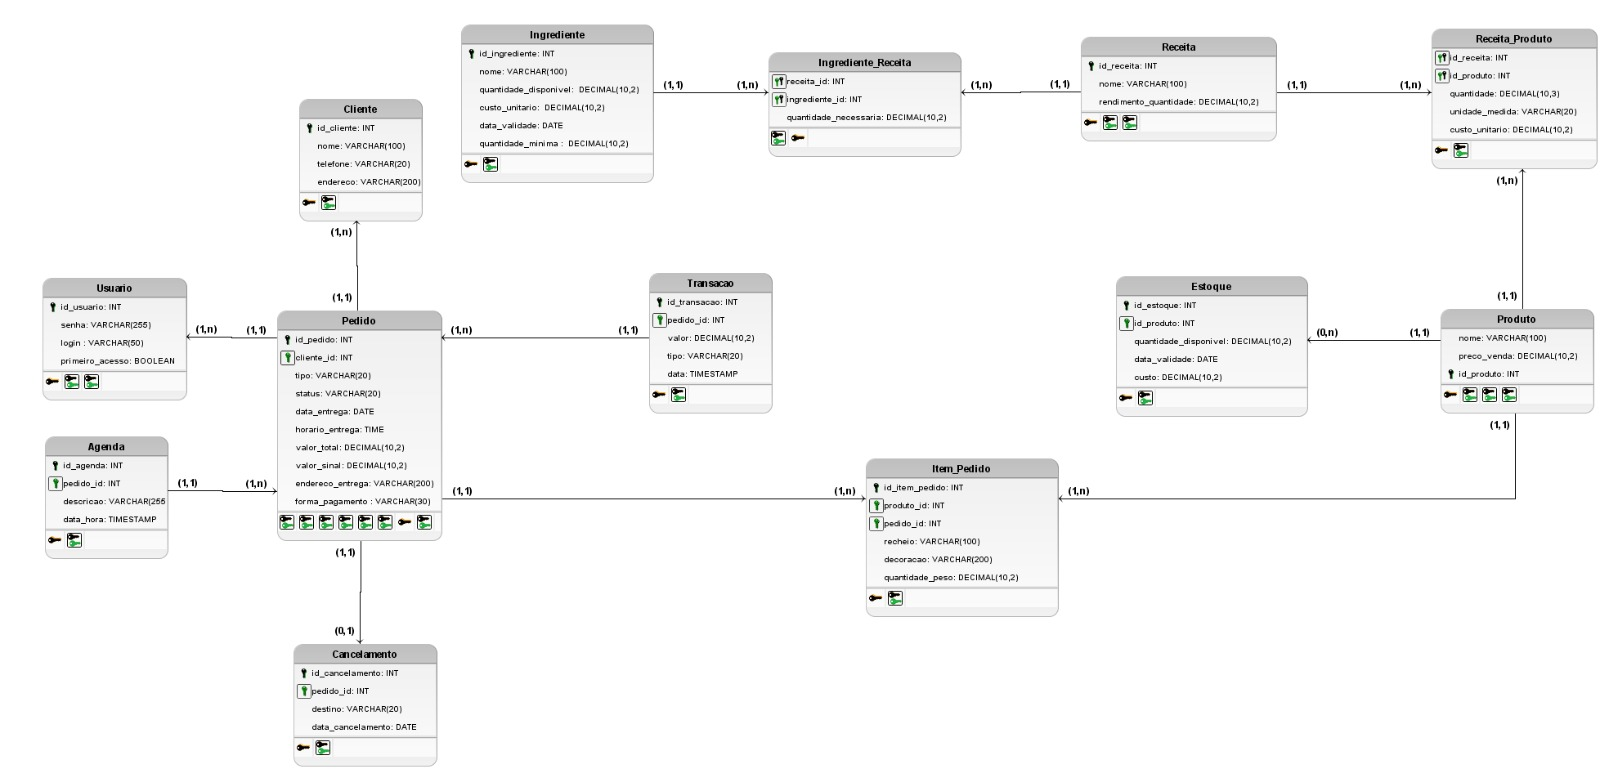
\includegraphics[width=\textwidth]{imagens/modelo_logico_dados.jpeg}
    \legend{Fonte: Elaborado pelos autores (2026).}
\end{figure}

\section{Projeto da Interface do Usuário}
A interface do Sistema Web Administrativo da Confeitaria Bom Gosto foi planejada para reunir as funcionalidades de gerenciamento em áreas específicas, facilitando a localização das informações e a execução das tarefas cotidianas.

A organização das telas considera as principais atividades da confeitaria, como registrar pedidos, consultar encomendas, acompanhar produtos e controlar o estoque. A separação dessas funcionalidades busca evitar que informações de naturezas diferentes fiquem concentradas em uma única tela, tornando a navegação mais organizada.

A tela principal está relacionada à visualização do calendário e à organização dos compromissos. Essa área permite consultar as datas associadas aos pedidos e acompanhar os horários previstos para entregas ou retiradas.

A página de pedidos é destinada à consulta e ao acompanhamento das encomendas já registradas. Sua finalidade é permitir que as informações sejam visualizadas e que o andamento dos pedidos seja acompanhado sem confundir essa área com a visualização do calendário.

A página de produtos reúne as informações dos itens produzidos ou vendidos pela confeitaria. Já o controle de estoque é realizado em uma área própria, permitindo consultar a disponibilidade dos produtos e organizar os registros relacionados aos ingredientes e às quantidades armazenadas, conforme a separação definida no sistema.

O projeto não prevê uma página independente para o gerenciamento de clientes. As informações necessárias ao atendimento são relacionadas aos próprios registros dos pedidos, conforme o escopo definido para a aplicação.
A organização da interface deve favorecer a clareza das informações e a facilidade de uso, considerando que o sistema será utilizado para apoiar tarefas administrativas e operacionais. A distribuição das funcionalidades em áreas específicas também busca tornar mais simples a identificação dos recursos disponíveis.

Segue a seguir o desenho da interface do sistema:

\begin{figure}[H]
    \centering
    \caption{\label{fig:prototipo_tela_login}Protótipo da Tela de Login}
    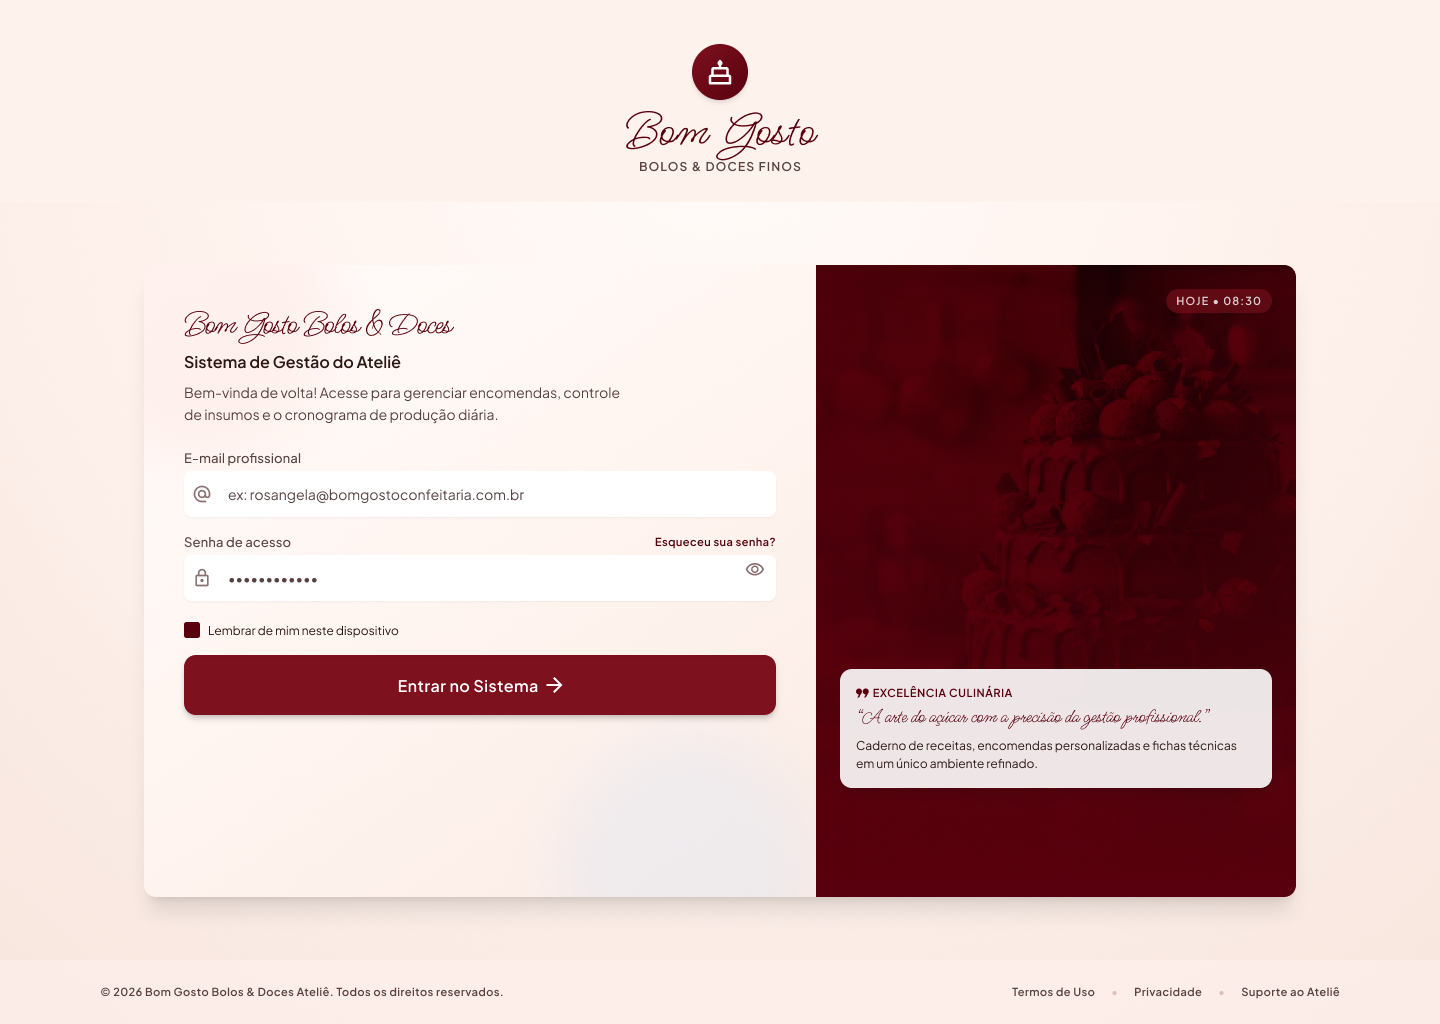
\includegraphics[width=\textwidth]{imagens/prototipo_tela_login.png}
    \legend{Fonte: Elaborado pelos autores (2026).}
\end{figure}

\begin{figure}[H]
    \centering
    \caption{\label{fig:prototipo_tela_recuperacao}Protótipo da Tela de Recuperação de Senha}
    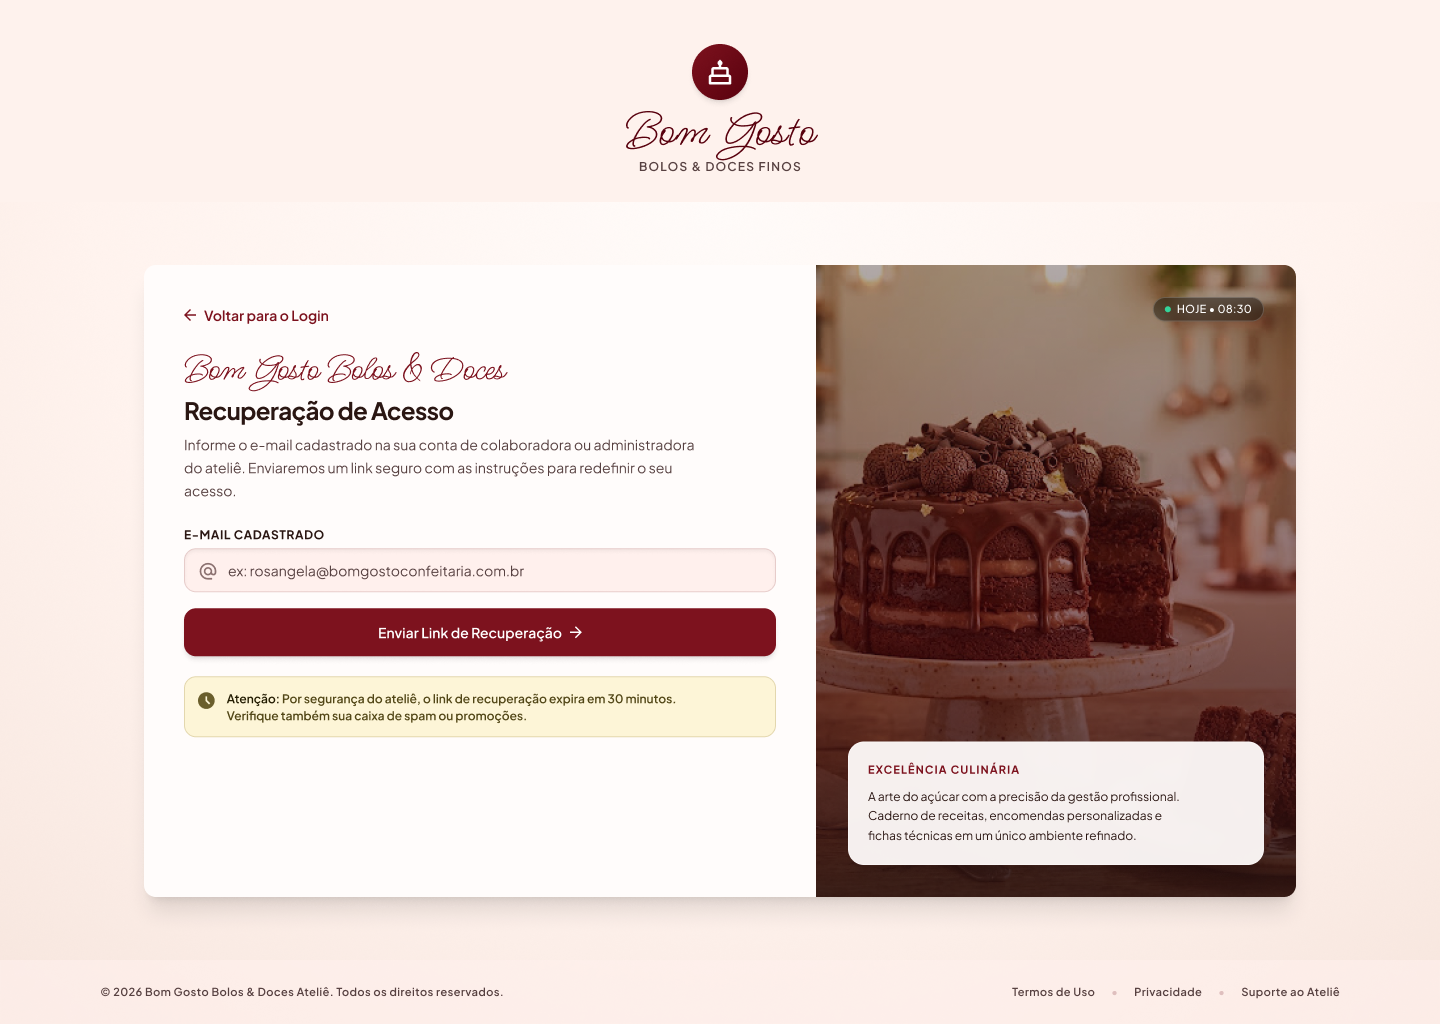
\includegraphics[width=\textwidth]{imagens/prototipo_tela_recuperacao.png}
    \legend{Fonte: Elaborado pelos autores (2026).}
\end{figure}

\begin{figure}[H]
    \centering
    \caption{\label{fig:prototipo_tela_inicial}Protótipo da Tela de Inicial}
    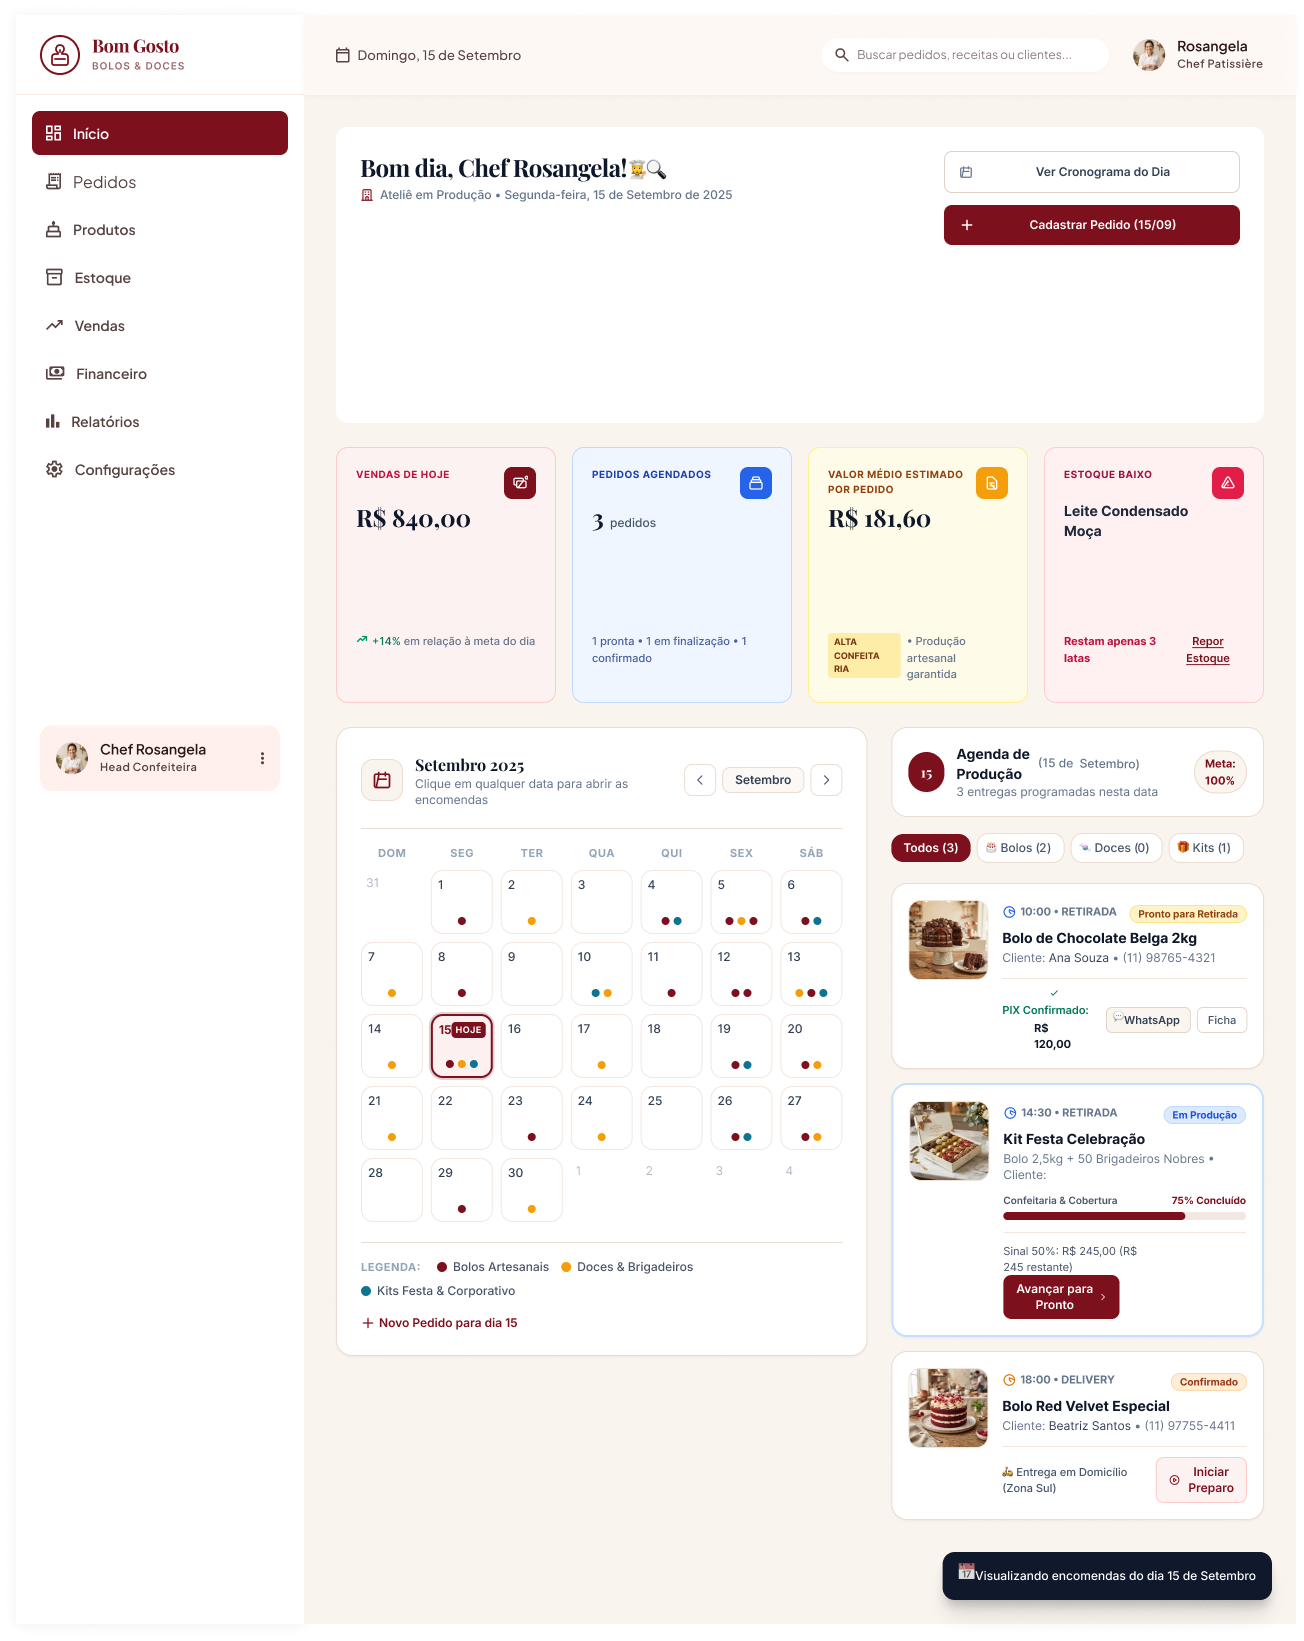
\includegraphics[width=\textwidth]{imagens/prototipo_tela_inicial.png}
    \legend{Fonte: Elaborado pelos autores (2026).}
\end{figure}

\section{Diagramas de Interação}
As interações entre os componentes do Sistema Web Administrativo da Confeitaria Bom Gosto ocorrem por meio de requisições HTTP baseadas no padrão arquitetural REST. O \textit{front-end} atua como cliente, consumindo os serviços e \textit{endpoints} disponibilizados pela API no \textit{back-end}.
Como exemplo validado na fase atual do projeto, a interação do Módulo de Autenticação se inicia quando o usuário insere suas credenciais na interface. O sistema envia a requisição para o \textit{endpoint /auth/login/} no servidor, que processa e consulta o banco de dados para validar a identidade de forma segura. Em caso de sucesso, o sistema verifica as regras de negócio de primeiro acesso e estabelece a sessão através do retorno de \textit{tokens} criptografados para o cliente.

%%\begin{figure}[H]
%%    \centering
%%    \caption{\label{fig:diagrama_sequencia}Diagrama de Sequência}
%%    
\includegraphics[width=\textwidth]{imagens/diagrama_pacotes.png}
%%    \legend{Fonte: Elaborado pelos autores (2026).}
%%\end{figure}

\section{Tecnologias Utilizadas}
O ambiente tecnológico seguido para o desenvolvimento do sistema tem como base uma arquitetura moderna e fácil de manter, organizada com base na abordagem de \textit{Monorepo} para facilitar a gestão do código-fonte de toda a aplicação em um repositório centralizado. As tecnologias que foram implementadas no desenvolvimento são:

\begin{itemize}
    \item \textbf{Interface gráfica (Front-End):} Utilização do framework Angular em conjunto com TypeScript, para a criação do visual e interação do cliente;
    \item \textbf{Lógica e API (Back-End):} Desenvolvimento utilizando a linguagem Python, utilizando o framework web Django e na biblioteca Django REST Framework para a construção e disponibilização das rotas e serviços;
    \item \textbf{Banco de dados:} Utilização do PostgreSQL como Sistema Gerenciador de Banco de Dados (SGBD) relacional, responsável por manter as entidades e a parte de dados do sistema;
    \item \textbf{Infraestrutura:} Adoção do Docker e Docker Compose para a conteinerização do ambiente de desenvolvimento, assegurando a padronização e o isolamento dos recursos;
    \item \textbf{Aprimoramento do código:} Emprego de ferramentas como Husky, Prettier e Commitlint para forçar regras do Conventional Commits e manter a estilização do código, suportados por esteiras de CI/CD automatizadas via GitHub Actions.
\end{itemize}

\section{Segurança e Controle de Acesso}

A segurança e o controle de acesso são aspectos importantes para um sistema que reúne informações administrativas, financeiras e operacionais. No caso da Confeitaria Bom Gosto, a aplicação deve considerar a necessidade de restringir o acesso às funcionalidades de gerenciamento e proteger os dados registrados durante a utilização do sistema.

O projeto prevê o acesso administrativo por uma pessoa autorizada, de acordo com as regras estabelecidas para a aplicação. Dessa forma, os mecanismos de controle de acesso devem ser compatíveis com as funcionalidades disponibilizadas e com o tipo de informação armazenada.

Entre os aspectos que precisam ser considerados estão a autenticação do usuário por meio de palavra chave, a restrição de acesso às áreas administrativas e a proteção das informações utilizadas pelo sistema, são utilizadas para impedir o uso indevido das funcionalidades. Além do controle de acesso, o sistema deve considerar a integridade dos registros. Por exemplo, a exclusão de um pedido deve exigir uma confirmação antes de ser concluída, conforme o requisito definido para o projeto. Essa medida busca reduzir a possibilidade de remoções acidentais de informações importantes.

É importante diferenciar as medidas previstas das que já estão implementadas. A presença de uma tela de \textit{login}, por exemplo, não comprova isoladamente que todas as áreas estejam protegidas ou que as sessões sejam tratadas de maneira segura. Por isso, a descrição final deve ser conferida com o código e com os testes realizados na aplicação.

Outro aspecto relevante para o acompanhamento dos pedidos é a representação de seus estados. O pedido pode passar por diferentes etapas ao longo do atendimento, desde seu registro até a conclusão ou o cancelamento. A definição desses estados permite compreender as transições possíveis e organizar o acompanhamento da encomenda.

%%\begin{figure}[H]
%%    \centering
%%    \caption{\label{fig:diagrama_estados}Diagrama de Estados}
%%    
\includegraphics[width=\textwidth]{imagens/diagrama_pacotes.png}
%%    \legend{Fonte: Elaborado pelos autores (2026).}
%%\end{figure}